\documentclass[times, utf8, zavrsni]{fer}
\usepackage{booktabs}
\usepackage{pdfpages}
\begin{document}

\thesisnumber{5709}

\title{Sustav za određivanje strukture teksta na temelju položaja pojedinih znakova}

\author{Herman Zvonimir Došilović}

\maketitle

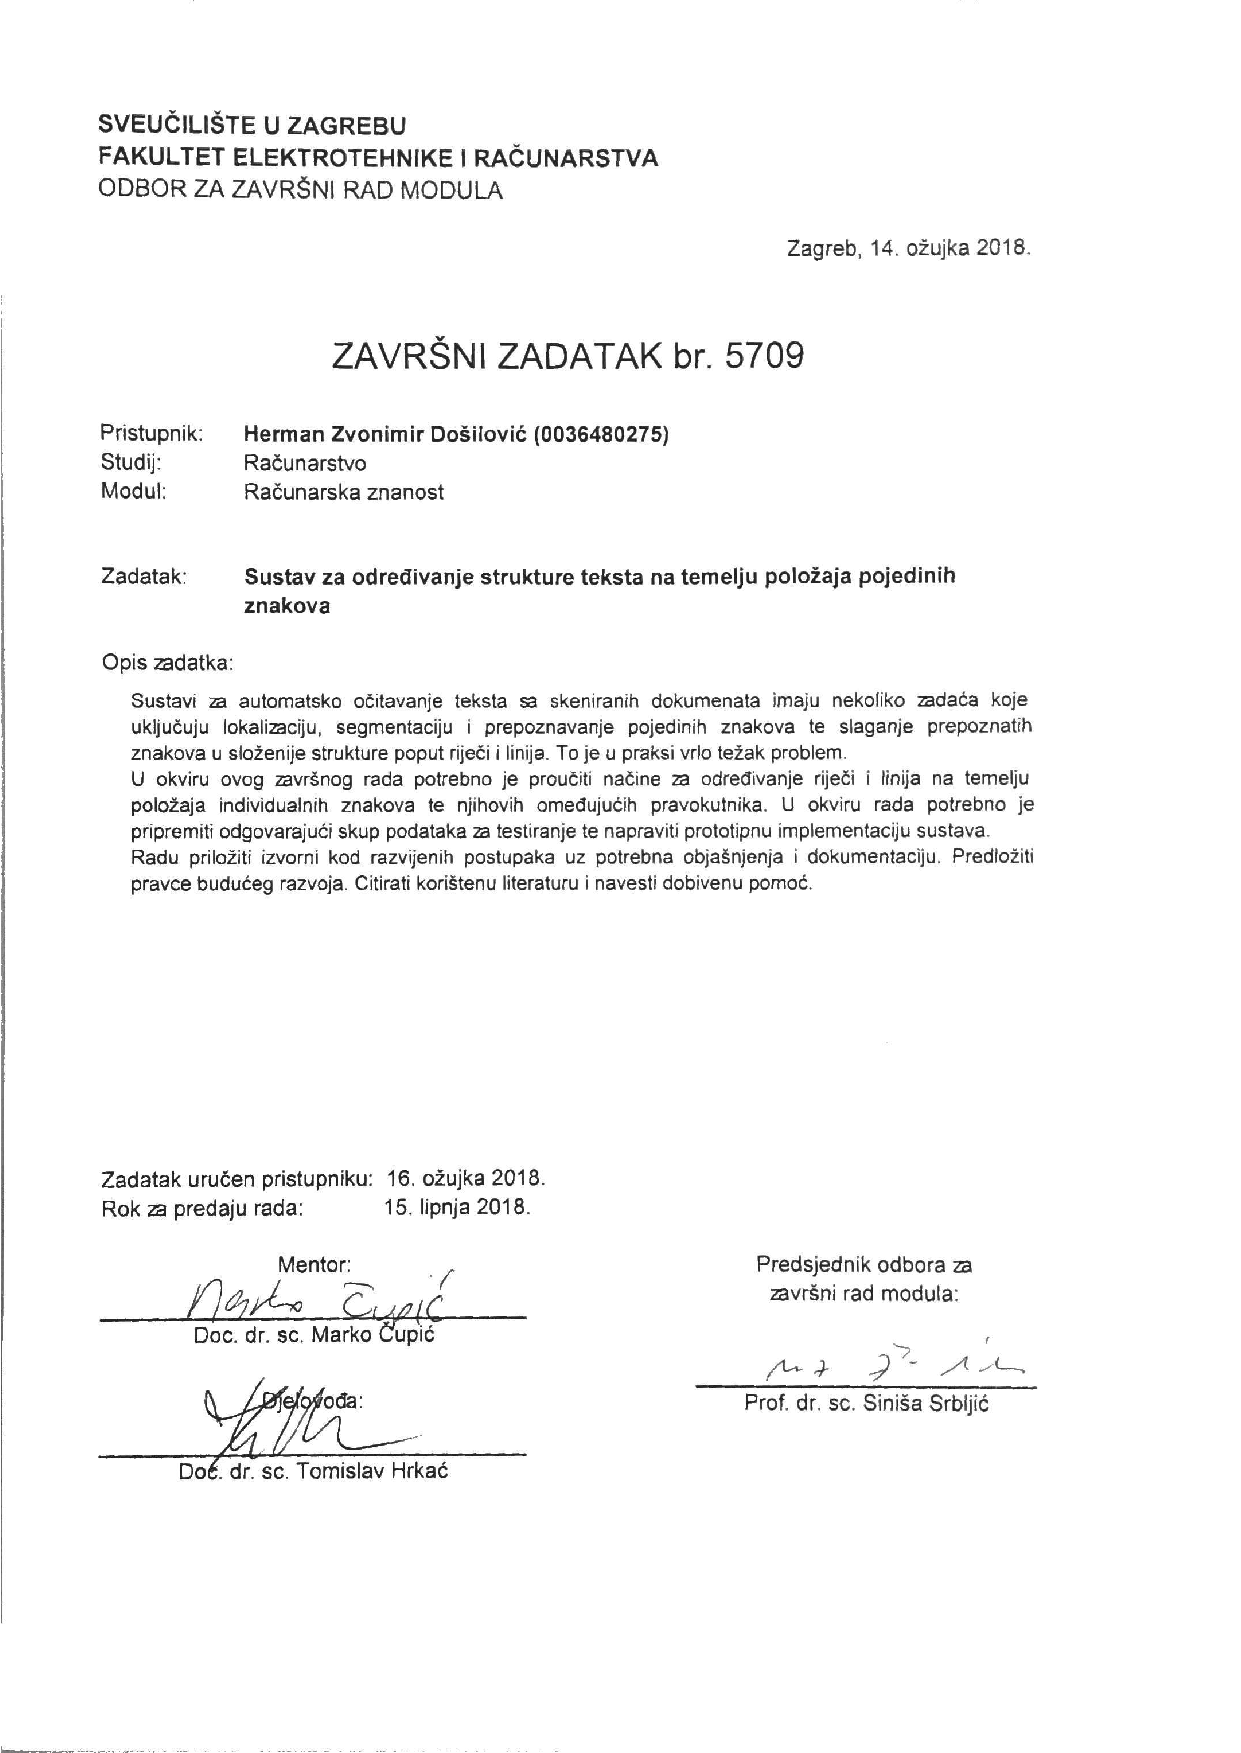
\includepdf[pages=-]{izvornik.pdf}

\zahvala{
    Zahvaljujem svom mentoru doc. dr. sc. Marku Čupiću na dozvoli za odabir vlastite teme i
    na strpljenju, poticaju i savjetima u razvoju rada.

    \

    Zahvaljujem tvrtki Microblink na danim sredstvima bez kojih ovaj rad ne bi bio moguć.
    Posebno zahvaljujem kolegama koji su me svojim bogatim znanjem i iskustvom
    usmjeravali u razvoju rada, a to su: Jurica Cerovec, Nenad Mikša, Boris Trubić, Igor Smolkovič i Ivan Jurin.
}

\zahvala{
    Tko hoće da među vama bude najveći, neka vam bude poslužitelj! I tko hoće da
    među vama bude prvi, neka bude svima sluga. - Mk 10,43-44
}

\tableofcontents

\chapter{Uvod}
\chapter{Optičko raspoznavanje znakova}
Sustav za optičko raspoznavanje znakova \engl{optical character recognition} (u daljnjem tekstu: OCR)
pretvara sliku tiskanog teksta u digitalizirani format kojim možemo jednostavno manipulirati na računalu.
Za razliku od ljudskog mozga, računalima nije lako prepoznati tekst i pojedine znakove teksta sa slike
zbog velike raznolikosti jezika, fonta i stila kojim tekst može biti napisan.
OCR je stoga vrlo zahtjevan problem i mnogo je istraživačkog truda uloženo u pokušaju
da se slike teksta pretvore u format koji računalo razumije. \citep{DBLP:journals/corr/abs-1710-05703}

\section{Primjene}

Osim tiskanog teksta, OCR sustavi koriste se i u prepoznavanju znakova rukom pisanog teksta.
Prepoznavanje znakova rukom pisanog teksta je teži problem od prepoznavanja tiskanog teksta \citep{DBLP:journals/corr/abs-1710-05703} zato jer
se oblik znakova i njihov način pisanja razlikuje kod svake osobe (npr. rukopis odrasle osobe potpuno je drugačiji od
rukopisa djeteta).
OCR sustave za detekciju rukom pisanih znakova možemo podijeliti na dvije potkategorije:
\emph{on-line} i \emph{off-line}. \emph{On-line} OCR sustavi detektiraju znakove dok
ih korisnici unose i to im omogućuje praćenje parametara poput: brzine pisanja, broj napravljenih poteza,
smjer pisanja, itd. \emph{Off-line} OCR sustavi izvode se nad jednom slikom na kojoj se nalazi
sav sadržaj nad kojim je potrebno napraviti detekciju. Takvi sustavi nemaju dodatne informacije koje imaju
\emph{off-line} sustavi i zato je detekcija znakova kompliciranija \citep{DBLP:journals/corr/abs-1710-05703}. Slika \ref{fig:math-example-01} prikazuje primjer rezultata
\emph{off-line} OCR sustava za detekciju rukom pisanih znakova.

\begin{figure}[htb]
    \centering
    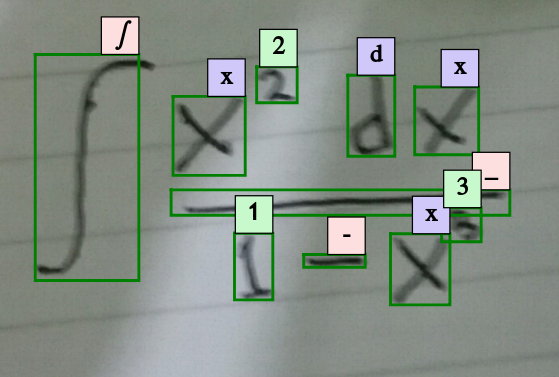
\includegraphics[height=4cm]{images/math-example-01.png}
    \caption{Rezultat \emph{off-line} OCR sustava za detekciju znakova rukom pisanog teksta.}
    \label{fig:math-example-01}
\end{figure}

OCR sustavi imaju široku primjenu i možemo ih pronaći primjerice u detekciji
znakova na registarskim pločicama \citep{DBLP:journals/corr/Saghaei16a}, \citep{DBLP:journals/corr/abs-1802-09567},
u detekciji znakova na tiskanim knjigama \citep{DBLP:journals/corr/abs-1802-10033},
\citep{Christy:2017:MDE:3172938.3075645} i
detekciji znakova na raznim dokumenatima \citep{DBLP:journals/corr/HarrajR15}. Na slici \ref{fig:receipt-example-01}
prikazan je primjer rezultata korištenja OCR sustava za detekciju znakova na računima iz trgovine.
Slika \ref{fig:book-example-01} prikazuje rezultat OCR sustava za detekciju znakova na tiskanim knjigama.

\begin{figure}[htb]
    \centering
    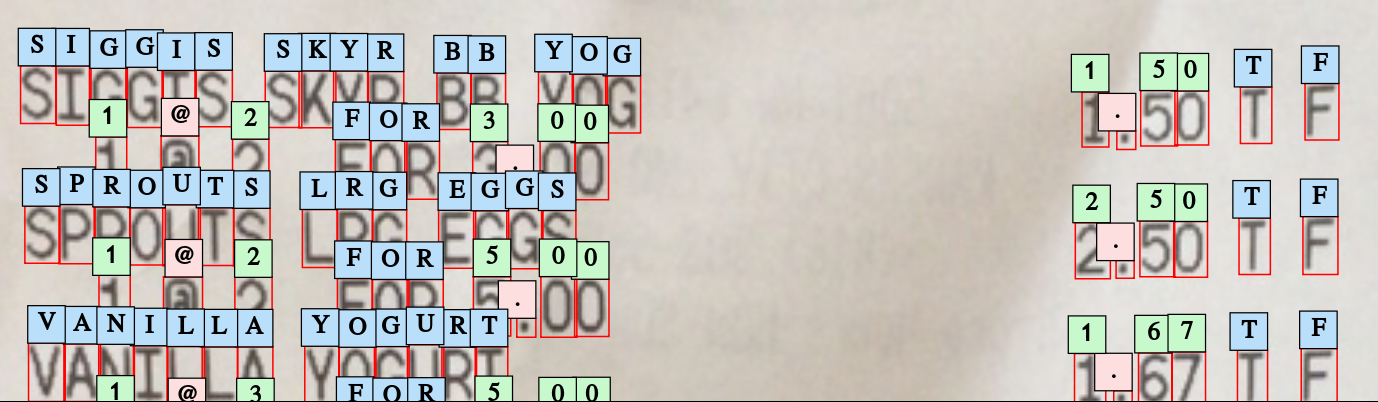
\includegraphics[height=4cm]{images/receipt-example-01.png}
    \caption{Rezultat OCR sustava za detekciju znakova na računima iz trgovine.}
    \label{fig:receipt-example-01}
\end{figure}

\begin{figure}[htb]
    \centering
    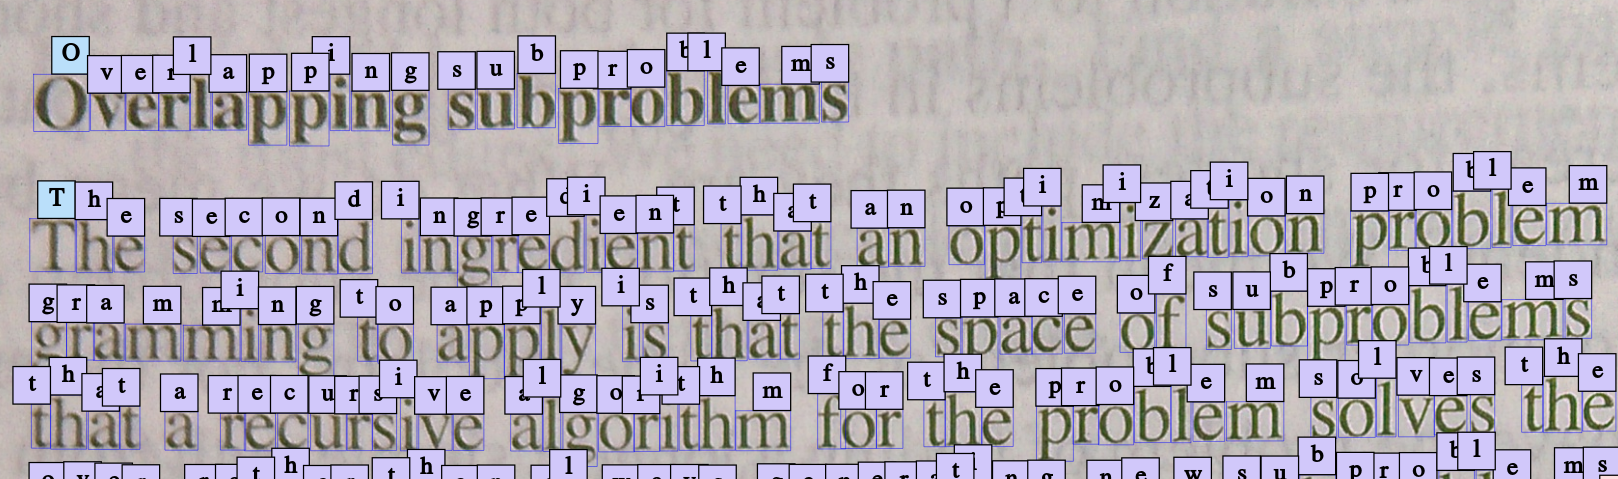
\includegraphics[height=4cm]{images/book-example-01.png}
    \caption{Rezultat OCR sustava za detekciju znakova na tiskanim knjigama.}
    \label{fig:book-example-01}
\end{figure}

\section{Proces izvođenja}

Optičko raspoznavanje znakova provodi se u nekoliko koraka \citep{DBLP:journals/corr/abs-1710-05703} \citep{kaur2016survey}:
\begin{enumerate}
    \item pribavljanje slike,
    \item pretprocesiranje,
    \item segmentacija znakova,
    \item izdvajanje značajki znakova,
    \item klasifikacija znakova i
    \item postprocesiranje.
\end{enumerate}

\subsubsection{Pribavljanje slike}

U prvom koraku OCR-a, pribavljanju slike, potrebno je pribaviti sliku nad kojom ćemo
provesti ostale korake. Sliku možemo pribaviti s raznih uređaja poput kamere fotoaparata,
mobilnog uređaja ili nekog drugog uređaja za digitalizaciju dokumenata \engl{scanner}.
Nakon prvog koraka, slika dokumenta nad kojim provodimo raspoznavanje znakova sastoji se
samo od slikovnih elemenata \engl{pixels} \citep{Vynckier:2018:HowOcrWorks}.
Slika \ref{fig:receipt-example-02} prikazuje primjer slike nad kojom možemo provesti
postupak raspoznavanja znakova. Primjetimo da slika može sadržiti pozadinu koju bi
OCR sustav trebao zanemariti.

\begin{figure}[htb]
    \centering
    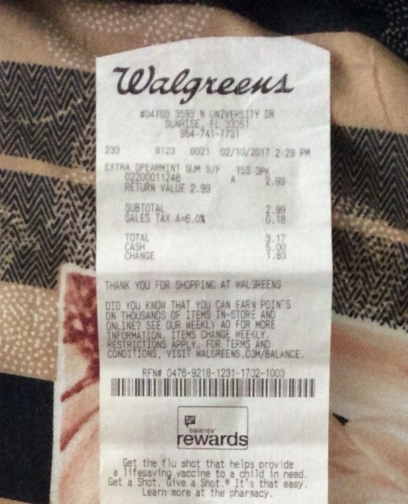
\includegraphics[height=8cm]{images/receipt-example-02.jpeg}
    \caption{Ulazna slika u OCR sustav pribavljena kamerom mobilnog uređaja.}
    \label{fig:receipt-example-02}
\end{figure}

\subsubsection{Pretprocesiranje}

U koraku pretprocesiranja slike provodimo niz morfoloških transformacija i filtra nad pribavljenom slikom.
Cilj ovog koraka je povećati kvalitetu slike i smanjiti informacije na slici. Binarizacija je jedan od
potkoraka pretporocesiranja koji slike u boji ili u nijansama sive pretvara u crno-bijele. Osim binarizacije
koriste se neke morfološke transformacije poput dilatacije, rezanja i skaliranja.
Slika \ref{fig:binarization} prikazuje primjer slike prije i nakon binarizacije. \citep{Gulan:2016:Bacherlor},
\citep{DBLP:journals/corr/abs-1710-05703}, \citep{Jurin:2017:Master}

\begin{figure}[htb]
    \centering
    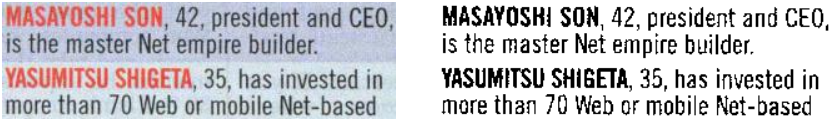
\includegraphics[height=2cm]{images/binarization.png}
    \caption{Prije binarizacije (lijevo) i nakon binarizacije (desno) \citep{Vynckier:2018:HowOcrWorks}.}
    \label{fig:binarization}
\end{figure}

\subsubsection{Segmentacija znakova}
\label{subsubsec:segmentacija}

Sljedeći korak, segmentacija znakova, je postupak segmentiranja slike u segmente unutar kojih se nalaze znakovi
koje želimo klasificirati. Jedna od pristupa segmentacije izvodi se s vrha prema dnu gdje se najprije
segmentiraju linije, zatim riječi i na kraju pojedini znakovi \citep{Jurin:2017:Master}, \citep{Vynckier:2018:HowOcrWorks}.
Prednost ovakvog pristupa je da uz lokaciju svakog znaka dobivamo i strukturu cijelog teksta, odnosno, znamo kojoj
liniji i kojoj riječi znak pripada. Nedostatak ovakvog pristupa je da ne postoje korekcijski mehanizmi kojima bismo
znak pridružili nekoj drugoj liniji ili riječi ako su prva dva koraka segmentacije linije ili riječi neispravni. \citep{Jurin:2017:Master}

Drugi pristupi poput \emph{ZICER OCR}\footnote{OCR sustav tvrtke \emph{Microblink}, \url{https://microblink.com}} sustava izravno
izvode segmentaciju cijele slike na području koji predstavljaju znakove. Prednost takvog pristupa je da
možemo detektirati znakove teksta u kojemu nema riječi i linija, kao što je na primjer matematički izraz.
Nedostatak takvog pristupa je da gubimo informaciju o strukturi teksta i zato postoji potreba za razvojem dodatnog sustava koji bi znakove
grupirao u riječi, a riječi u linije \citep{Jurin:2017:Master}.
Slika \ref{fig:segmentation} prikazuje rezultat segmentacije pojedinih znakova.

\begin{figure}[htb]
    \centering
    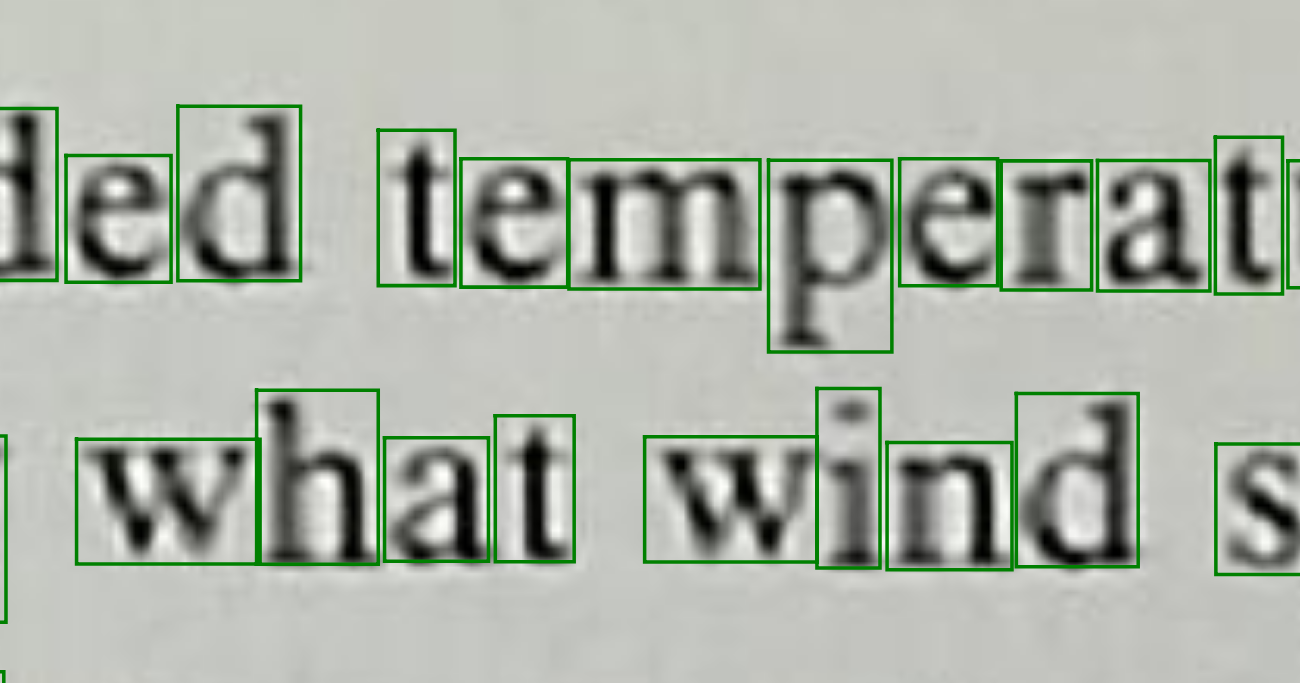
\includegraphics[height=4cm]{images/segmentation.png}
    \caption{Segmentacija znakova.}
    \label{fig:segmentation}
\end{figure}

\subsubsection{Izdvajanje značajki}

Izdvajanje značajki pojedinog znaka podrazumjeva odabir značajki prema kojima će
se jedinstveno klasificirati svaki znak. Značajke poput geometrijskog oblika ili
statističkih svojstava mogu biti uzete u obzir prilikom klasifikacije. Važno područje istraživanja pripada
razmatranju koje i koliko značajki je potrebno uzeti u obzir za kvalitetnu i ispravnu
klasifikaciju. \citep{DBLP:journals/corr/abs-1710-05703}

\subsubsection{Klasifikacija}

Klasifikacija je najvažniji korak optičkog raspoznavanja znakova \citep{verma2012survey}
koji koristi izdvojene značajke za određivanje klase pojedinog znaka \citep{lehal1999feature} \citep{kaur2016survey}.
Statistički pristupi klasifikacije koriste diskriminativne funkcije za određivanje klase znaka \citep{DBLP:journals/corr/abs-1710-05703},
a u novije vrijeme koriste se duboke neuronske mreže \citep{Jurin:2017:Master}.
Neki od statističkih pristupa su: Bayesov klasifikator, klasifikator stablom odluke, umjetne neuronske mreže i
metoda k-najbližih susjeda \citep{DBLP:journals/corr/abs-1710-05703}.

2012. godine Krizhevsky i suradnici \citep{krizhevsky2012imagenet} objavili su rad koji je
označio prekretnicu u klasifikaciji i lokalizaciji objekata \citep{Jurin:2017:Master}. Slika
\ref{fig:deep-example-01} prikazuje arhitekturu \emph{AlexNet} koja je pobijedila na natječaju
\emph{ImageNet 2012} u području klasifikacije objekata. \citep{Jurin:2017:Master}

\begin{figure}[htb]
    \centering
    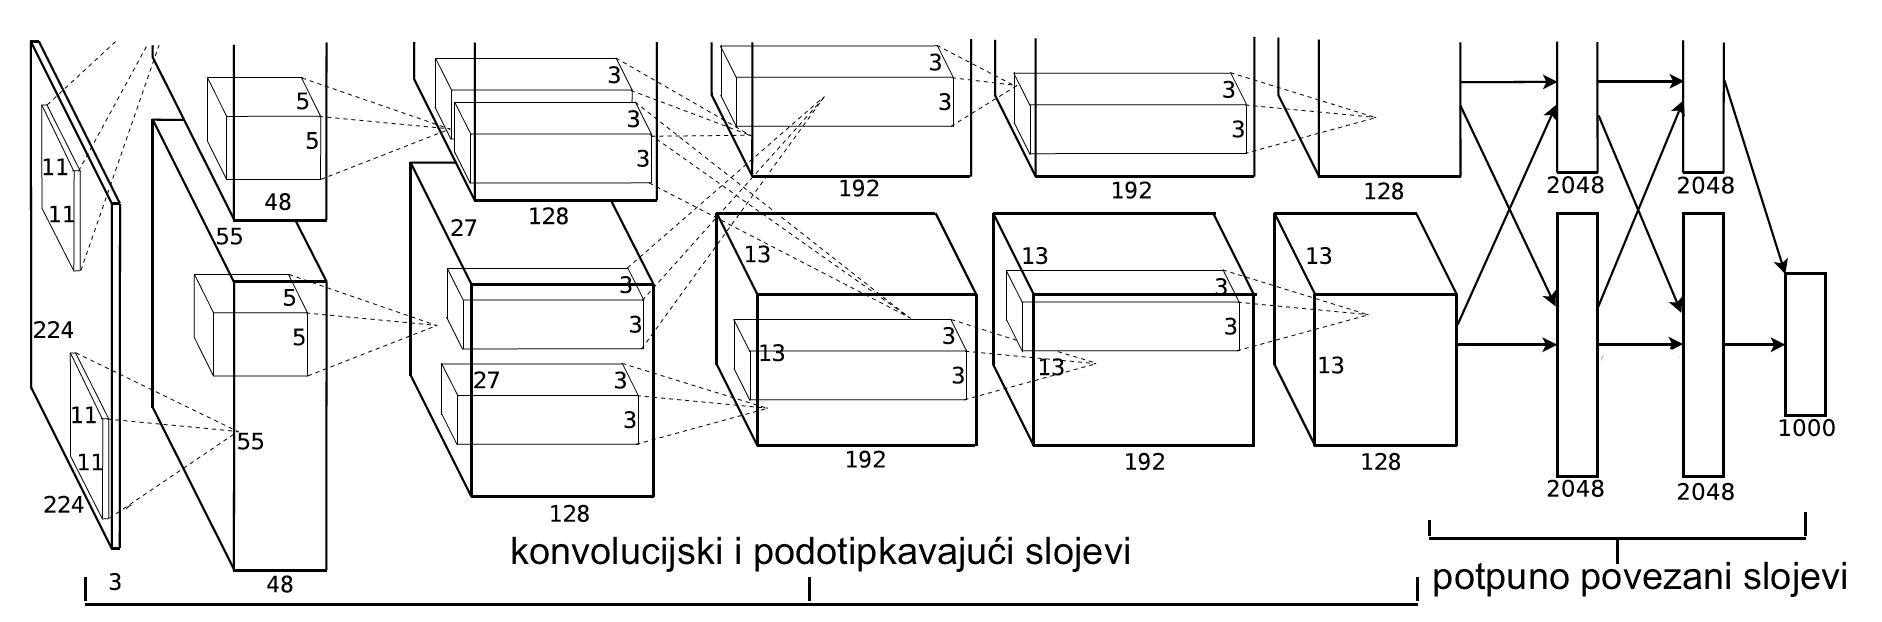
\includegraphics[height=5cm]{images/deep-example-01.png}
    \caption{Arhitektura \emph{AlexNet} \citep{Jurin:2017:Master}}
    \label{fig:deep-example-01}
\end{figure}

\subsubsection{Postprocesiranje}

Nakon klasifikacije znakova slijedi njihovo postprocesiranje koje se koristi kako
bi se poboljšali rezultati OCR-a. Jedan od pristupa postprocesiranja koristi rezultate
više različitih klasifikatora koji mogu biti korišteni slijedno, paralelno ili hijerarhijski.
Nakon toga rezultati klasifikatora se kombiniraju različitim pristupima. \citep{DBLP:journals/corr/abs-1710-05703}
Kao što je spomenuto u \ref{subsubsec:segmentacija} segmentacija koja se ne provodi s vrha prema
dnu nema informaciju o strukturi teksta i zato je potrebno razviti dodatan
\textbf{sustav za određivanje strukture teksta na temelju položaja pojedinih znakova}.

Schulz i suradnici \citep{schulz2017multi} 2017. godine predstavili su arhitekturu
tzv. \emph{post-correction} OCR sustava kojim su pokazati na koji način su
adaptirali generički sustav za postprocesiranje OCR rezultata koristeći domensko znanje
za konkretan problem koji su rješavali. Ovim pristupom ostvarili su bolje rezultate
za konkretni problem nego što su ostvarili koristeći postojeći generički sustav za
postprocesiranje OCR rezultata.

\begin{figure}[htb]
    \centering
    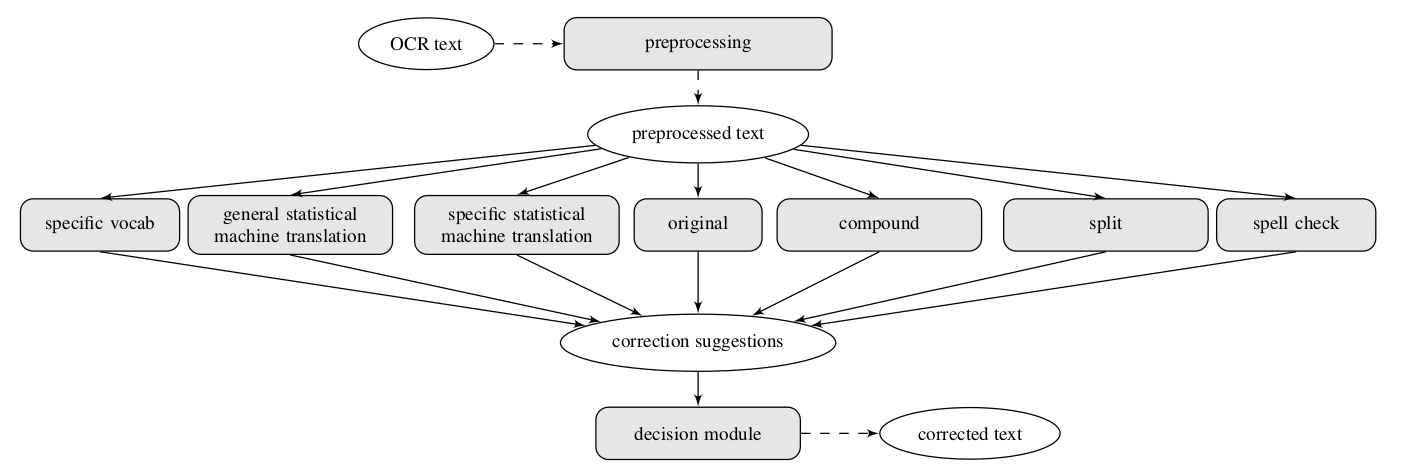
\includegraphics[height=5cm]{images/post-correction-example-01.png}
    \caption{Arhitektura \emph{post-correction} OCR sustava \citep{schulz2017multi}}
    \label{fig:post-correction-example-01}
\end{figure}

\chapter{Zaključak}
\bibliography{literatura}
\bibliographystyle{fer}

\begin{sazetak}

\kljucnerijeci{}
\end{sazetak}

\engtitle{Text Layout Analysis System Based on Individual Character Positions}
\begin{abstract}

\keywords{}
\end{abstract}

\end{document}
